\section{Iontové procesy}

\subsection{Příklad 1.2.1}
\begin{zadani}
    Srovnejte základní vlastnosti elektronů a iontů.
\end{zadani}

Elektrony mají vždy záporný náboj a jsou obecně podstatně lehčí a menší než ionty. Díky své nízké hmotnosti se mohou pohybovat velmi vysokými rychlostmi blížícími se rychlosti světla. 

Ionty mohou mít kladný i záporný náboj a jsou větší a těžší. Oproti elektronům mohou také tvořit chemické reakce (jelikož se jedná o celé ionizované atomy nebo molekuly). Lze je použít například i pro depozici tenkých vrstev.


\subsection{Příklad 1.2.2 - výpočet}
\begin{zadani}
    Stanovte maximální koncentraci implantovaných iontů bóru do 
    monokrystalu křemíku ve vzdálenosti středního doletu iontů  Rp od 
    povrchu destičky a koncentraci iontů ve vzdálenosti  Rp \(\pm \Delta\)Rp a na 
    povrchu monokrystalu.  \(\Delta\)Rp  je střední kvadratická odchylka. Zjištěný  
    koncentrační profil naznačte graficky. Celková dávka  Q = 1018 m-2 při  
    energie iontů  100 keV
\end{zadani}


Pro implantaci bóru do křemíku při energii iontů \qty{100}{keV} platí:

Rp = \qty{0,2994}{\micro\meter} a \(\Delta\)Rp = \qty{0,0710}{\micro\meter}

Pro stanovení maximální koncentrace vyjdeme z následujícího vztahu:
\begin{align*}
  N_{max} &= \frac{Q}{\sqrt{2\pi \Delta R_{p} } } \\
  N_{max} &= \frac{\num{10e18}}{\sqrt{2\pi \num{0,0710e-6} } } \\
  N_{max} &= \qty{1,49e21}{\per\meter\cubed}
\end{align*}

Jak by vypadal koncentrační profil v závislosti na vzdálenosti od povrchu můžeme vidět na obrázku~\ref{fig:img-profil}

\begin{figure}[h!]
  \centering
  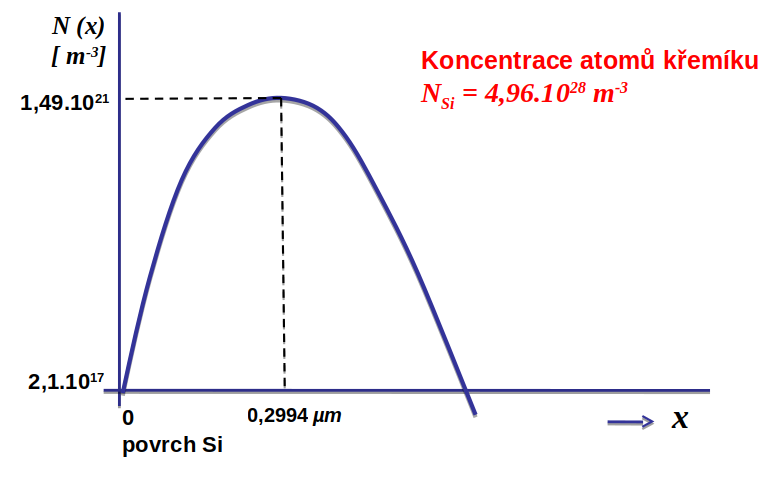
\includegraphics[width=0.6\textwidth]{img/profil.png}
  \caption{Závislost koncentrace dopantů na hloubce resp. vzdálenosti od povrchu.}
  \label{fig:img-profil}
\end{figure}

